\documentclass[12pt]{article}
\usepackage[english]{babel}
\usepackage{natbib}
\usepackage{url}
\usepackage[utf8x]{inputenc}
\usepackage{amsmath}
\usepackage{graphicx}
\graphicspath{{images/}}
\usepackage{parskip}
\usepackage{fancyhdr}
\usepackage{listings}
\usepackage{subfigure}
\usepackage{csvsimple}
\usepackage{longtable}
\usepackage{vmargin}
\setmarginsrb{3 cm}{2.5 cm}{3 cm}{2.5 cm}{1 cm}{1.5 cm}{1 cm}{1.5 cm}
\usepackage{color}
 
\definecolor{codegreen}{rgb}{0,0.6,0}
\definecolor{codegray}{rgb}{0.5,0.5,0.5}
\definecolor{codepurple}{rgb}{0.58,0,0.82}
\definecolor{backcolour}{rgb}{0.95,0.95,0.92}
 
\lstdefinestyle{mystyle}{
    backgroundcolor=\color{backcolour},   
    commentstyle=\color{codegreen},
    keywordstyle=\color{magenta},
    numberstyle=\tiny\color{codegray},
    stringstyle=\color{codepurple},
    basicstyle=\footnotesize,
    breakatwhitespace=false,         
    breaklines=true,                 
    captionpos=b,                    
    keepspaces=true,                 
    numbers=left,                    
    numbersep=5pt,                  
    showspaces=false,                
    showstringspaces=false,
    showtabs=false,                  
    tabsize=2
}
 
\lstset{style=mystyle}

\title{Multivariate Report}								% Title
\author{Gawronsky, Marcus \newline Singo, Una}
\date{\today}											% Date

\makeatletter
\let\thetitle\@title
\let\theauthor\@author
\let\thedate\@date
\makeatother

\pagestyle{fancy}
\fancyhf{}
%\rhead{\theauthor}
\lhead{\thetitle}
\cfoot{\thepage}
\setcounter{secnumdepth}{0}

\begin{document}

%%%%%%%%%%%%%%%%%%%%%%%%%%%%%%%%%%%%%%%%%%%%%%%%%%%%%%%%%%%%%%%%%%%%%%%%%%%%%%%%%%%%%%%%%

\begin{titlepage}
	\centering
    \vspace*{0.5 cm}
    
\includegraphics[scale = 0.75]{UCT.jpg}\\[1.0 cm]	% University Logo
    \textsc{\LARGE University of Cape Town}\\[2.0 cm]	% University Name
	\textsc{\Large STA5069Z}\\[0.5 cm]				% Course Code
	\textsc{\large Multivariate Statistics}\\[0.5 cm]				% Course Name
	\rule{\linewidth}{0.2 mm} \\[0.4 cm]
	{ \huge \bfseries \thetitle}\\
	\rule{\linewidth}{0.2 mm} \\[1.5 cm]
	
	\begin{minipage}{0.4\textwidth}
		\begin{flushleft} \large
			\emph{Authors:}\\
			\theauthor
			\end{flushleft}
			\end{minipage}~
			\begin{minipage}{0.4\textwidth}
			\begin{flushright} \large
			\emph{Student Number:} \\
            GWRMAR002 SNGUNA003									% Your Student Number
            
		\end{flushright}
	\end{minipage}\\[2 cm]
	
	{\large \thedate}\\[2 cm]
 
	\vfill
	
\end{titlepage}

%%%%%%%%%%%%%%%%%%%%%%%%%%%%%%%%%%%%%%%%%%%%%%%%%%%%%%%%%%%%%%%%%%%%%%%%%%%%%%%%%%%%%%%%%


\begin{abstract}


\noindent Variational Autoencoders (VAEs) are a class of generative artificial neural network commonly used for dimensionality reduction in machine learning applications.  In this paper, we implement a stable Variational Autoencoder and benchmark its performance against traditional methods in multivariate statistics using common open data sets. We build on our implementation with two experiments; the first is an application to noncolumnar data in the medical field, and the second is an original generative sampling problem. 

\end{abstract}

%%%%%%%%%%%%%%%%%%%%%%%%%%%%%%%%%%%%%%%%%%%%%%%%%%%%%%%%%%%%%%%%%%%%%%%%%%%%%%%%%%%%%%%%%

\newpage
\tableofcontents
\pagebreak

%%%%%%%%%%%%%%%%%%%%%%%%%%%%%%%%%%%%%%%%%%%%%%%%%%%%%%%%%%%%%%%%%%%%%%%%%%%%%%%%%%%%%%%%%
\section{Literature Review}
Variational Autoencoders (VAEs) are a class of generative artificial neural network commonly used for dimensionality reduction in machine learning applications.  The technique extends on the application of traditional autoencoders and deep belief networks by introducing techniques from Variational Bayesian Methods.  

An autoencoder consists of two neural networks, an encoder network and decoder network. The encoder network takes an input and produces a lower-dimensional representation of the data. The decoder network takes the lower-dimensional representation of the data and learns a reconstruction of the data back into its original vector-space. These neural networks can have a varying number of hidden-layers, activation functions and neurons to learn non-linear representations of the data \citep{Bengio2007, Bengio2013}.  

Variational Bayesian Methods are a class of techniques used in approximating intractable integrals found in Bayesian Modeling.  Using an approximate distribution, $q^\star(x)$, a loss function is used to minimize the difference between the approximate distribution and true posterior.  This loss function is often chosen to be the Evidence Lower Bound (ELBO) or Kullback–Leibler divergence and is weighted in the optimization procedure to ensure the validity of the applied approximate distribution.   

The Variational Autoencoder aims to extend on encoder-decoder model architectures by placing distributional assumptions on the low-dimensional latent space.  By making this assumption, these models can be generative, allowing one to sample data across a complex data manifold.  Figure \ref{fig:Bench1} aims to show the basic architecture of a VAE. The input data $\mathbf{X}$ is assumed to be an $i.i.d.$ high dimensional dataset and the latent variables are denoted as $\mathbf{z}$ are assumed to follow an unobservable distribution. The encoder network is defined as the conditional probability distribution $q_{\theta}(\mathbf{z}|\mathbf{x})$ and outputs estimates to $q_{\theta}(\mathbf{z}|\mathbf{x})$ which is assumed to follow a parametric probability distribution. Using the estimated parameters from the encoder neural network, sample values of $\mathbf{z}$ are computed and used as an input to the decoder neural network $p_{\theta}(\mathbf{x}|\mathbf{z})$ which outputs estimates to the conditional distribution $p_{\theta}(\mathbf{x}|\mathbf{z})$ which can be used to sample values of $\mathbf{x}$. A key aspect to the model is the distributional assumption on the latent space. While several methods can be used to ensure the model distributional assumption, the original authors include the Kullback–Leibler divergence into the loss function of the model to ensure a distribution over latent variable which is approximately standard normal \citep{vaeBayes, zhao2017infovae, tolstikhin2017wasserstein}.  
\newline

\noindent Using these techniques, Variational Autoencoders provide a flexible method which can be applied to solve a wide range of problems across domains. In the original paper,  \cite{vaeBayes} use the popular MNIST dataset to both embed and generate new images of handwritten digits. A significant number of subsequent research on VAEs has focused on the learning latent distributions of images and generating new images. Generative Adversarial Networks are a popular example of such research outputs where the objective is to generate fake images that appear to be authentic to human observers \citep{Goodfellow2014}.  \newline 
Apart from image generation VAEs have been shown to solve anomaly detection problems. \cite{An2015} propose a method using the reconstruction probability from a variational autoencoder to identify outliers. Their experimental results show that this method outperforms traditional auto-encoder and principal components based methods.\\




\section{Setup}
Code for this assignment was written in Python version 3.7.1, using a random seed of 1234, a full list of the Python dependencies are listed in the appendencies in a YML file.  This can be used, along with the code \footnote{The code is accessible on github: https://github.com/marcusinthesky/super-spirals.git}, to reproduce the analysis provided.  


\section{Data}
Five open data sets and two simulated are used in this assignment. Of the open data sets, three are column-oriented and two audio based. This section will provide a short description of the data, its source, and some information about its characteristics.

\subsection{Iris Flowers}

The Iris flower dataset \citep{fisher_1936} measures 4 distinguishing features of three related species of Iris flowers, Setosa, Veriscolour and Virginica. It contains 150 observations with 5 variables, a classifier, the sepal length, sepal width, petal length and petal width. It is commonly used as an introduction to solving classification, clustering and dimensional reduction problems. 

\subsection{Wine}
The Wine dataset \citep{aeberhard_coomans_de_vel_1992} contains results from a chemical study of wine grown in the same region in Italy but grown by three different farmers. The data contains 178 observations, 13 predictive numerical features that measure chemicals properties.

\subsection{Breast Cancer}
The Breast Cancer \citep{street_wolberg_mangasarian_1993} data contains features computed from an image of a fine needle aspirate (FNA). Fine-needle aspiration (FNA) is a diagnostic procedure used to investigate lumps. Using a fine needle cells from the lump are extracted and studied under a microscope, from the image 30 features can be measured that characterise the mass and distinguish it from being Benign or Malignant. 

\subsection{Heartbeats Audio Recordings}
The Heartbeats dataset \citep{pascal-chsc-2011} is an audio data set that contains recordings of heartbeats from a two stethoscope apps. There are four classes of audio, artifact, extrahls, murmer and normal. The data set was originally created to identify S1 (dub) and S2 (dub) sounds and classify beats into one of the four classes.  
\newpage
\section{Analysis}
In the literature, we have seen a variety of VAE implementations to solve multivariate problems. In this section, we present benchmark the applications of VAEs to problems in dimensionality reduction for clustering and manifold learning. We also demonstrate the application of VAEs to real-world datasets from the medical field and test an original generative modelling example. 
\subsection{Benchmarking}
\subsubsection{Dimensionality reduction for clustering}
Clustering high dimensional data can be difficult as regions in the space become increasingly sparse and data tends to equidistance. To solve this 'curse of dimensionality', dimensionality reduction is often applied in order to control for the correlation between dimensions and to aid in identifying separable clusters. We explored the feasibility of using a VAE to map high dimensional data to a lower-dimensional space for use in clustering.

We trained VAEs, on the Iris, Cancer and Wine dataset and visualised their latent space. As a benchmark, we also implemented Principal Component Analysis (PCA), Independent Component Analysis (ICA) and Kernal Principal Component Analysis (KPCA). Figures \ref{fig:benchirislatent}, \ref{fig:benchcancerlatent} and \ref{fig:benchwinelatent} show the input data mapped to the latent space, point is coloured according to class. 

By observation, the PCA for all data sets produces latent spaces with significantly more variation within classes compared to the other models. The KPCA seems to be the most consistent across datasets in the way that it maps inputs to the latent space. The ICA seems to produce tightly condensed clusters that will be difficult to separate.

To get a quantitative sense of the feasibility of clustering data in the latent space, we needed to create a ground truth clustering measure. We used the original class labels computed silhouette scores. These scores summarise the level of cohesion within clusters and separation between clusters. Scores range from -1 to 1, and high values mean that objects of a cluster are cohesive and well separated to other clusters.\\

Figure \ref{fig:clustering} shows the silhouette scores for each method trained on Iris, Cancer and Wine. The KPCA methods consistently produce scores that are above 0.4. The KPCA(RBF) method produces the highest score with the Wine dataset. The VAEs performance varies significantly between datasets. The VAE(Tanh) performs the best when trained on the Iris and Cancer dataset but is the weakest performer on the wine dataset. The VAE(ReLu) only performs well with the Cancer dataset and performs poorly with the Iris and Wine dataset. It appears that the VAEs performance is quite sensitive to the type of activation function used in training. Given the lack of consistent performance, the feasibility of using a VAE for efficient dimensionality reduction as a pre-processing step for clustering is questionable. While methods such as KPCA produced consistent results, there is a trade-off. The KPCA method is are basis expansion methods, and so time complexity is likely to be a problem.

%The first step of a VAE is to encode an observation $\mathbf{x} \in \mathbb{R} ^{n}$ to two a lower dimensional latent space that maintains the structure of the input data. However, instead of encoding data to a specific point in the latent space, a distribution over the latent space is learnt. In practice the distribution of the latent space is Gaussian. Consequently, the encoder is trained to output two vectors, a vector of means, $\mathbf{\mu}$ and a vector of standard deviations $\mathbf{\sigma}$. These parameters are used to sample from the Gaussian distribution and are passed to the decoder. Figure \ref{fig:Bench1} shows how information is passed through the network. \newline
%By training a network to learn a two dimensional latent space, we can visualise how the input space is mapped the two mean components. For observations of the same class, we expect their encoding to be close to each other and not overlap with other observations of different classes. 



\subsubsection{Manifold Learning}
Linear projection methods such a PCA  are quite useful at finding low dimensional structure when the data lies in an approximately linear subspace called a manifold.  A manifold is a topological space that resembles a euclidean space within the neighbourhood of a point in the manifold space. When the input data lies on a non-linear manifold, linear methods fail to maintain its local structure such as geodesic distances.  Given that neural networks are well suited to operate on non-linear data, we tested whether a VAE could learn a non-linear 2-dimensional manifold and benchmarked it to other manifold learning techniques, more specifically, PCA, Isomaps, Locally Linear Embedding (LLE), Multidimensional Scaling (MDS), Spectral Embedding and t-distributed Stochastic Neighbor Embedding (t-SNE). While we do not expect the Variational Autoencoder to capture manifold learning tasks, we aim to identify the robustness of the method to highly non-linear data as compared to PCA.  


We generated two input datasets, an S-curve and a Swiss Roll in $\mathbb{R}^{3}$ and coloured points according to a rainbow colour spectrum to offer visual guidance. The learned manifolds are presented in figures \ref{fig:scurve} and \ref{fig:swissroll}. \\

For the S-Curve, the Isomap seems to produce the best representation of the manifold. The method is capable of preserving the clusters in the input space, and the curvature does not appear to hinder its ability to unroll the S. The Spectral Embedding also produces a decent representation, the difference here is that it reduces the variation in observations of the same colour.  The VAEs are unable to learn the manifold; both seem to struggle to capture the geodesic distances necessary to produce lower-dimensional representation. The  Relu activation suffers the most as some of the red colour observations are not represented in the latent space. The Tanh performs slightly better and similar to the MDS as it is capable of preserving the clusters of the input space.\\

The Swiss roll problem adds a layer of complexity by introducing non-linear spiralling. The Isomap and TSNE produce a good representation of the manifold, once again being able to preserve clusters and deal with curvature. Both VAEs struggle to learn the manifold, the geodesic distances are not accounted for, but they are capable of maintaining some form of clustering. The Relu activation improves slightly as all observations are represented in the latent space. The Tanh activation is close as we can see that it is close at representing the spiral structure of the data. \\

While in both examples the Isomap and the TSNE methods produce favourable results, they are known to be the most computationally expensive and so they may not be well suited for large datasets. On the other hand, VAEs have failed to learn the manifold but allow for non-linear representations that are superior to PCA and MDS. 
\newpage








% if its non linear, maybe it can capture the major sources of variation, so we want to analyise its performance on manifiold learning tasks.



%As a departure point we trained a simple VAE on the Iris dataset. The network architecture is presented in table \ref{tab:iris}. The encoder maps a single Iris vector $\mathbf{x} \in \mathbb{R} ^{4}$ through the network to lower dimensional latent space in $\mathbb{R} ^{2}$, characterised by a bi-variate Gaussian distribution. The decoder maps the latent space back to its original data space and the model is trained to minimise the reconstruction error. \\

%A well trained model is expected to map the input data to a latent space such that input observations of the same class are spatially close to each other while objects of different classes are well separated. Figure \ref{fig:irislatent} shows the mapping of the Iris input data to the latent space. For nost of the observations the VAE is able to map to the a separable latent space. However, it seems that it has difficulty separating Veriscolour and Virginica classes. The inability to separate classes in the latent space means that the decoder will struggle to reconstruct observations efficiently. In the Benchmark section we will explore how this reconstruction loss compares to other well known dimensionality reduction algorithms. 


%\begin{table}[h!]
%    \centering
%    \begin{tabular}{|c|c|c|c|}
%        \hline
%         & Hidden Layers & Activation Function   \\
%         \hline
%         Encoder & 5, 2 & tanh   \\
%         Decoder & 2, 5 & tanh \\
%         \hline
%    \end{tabular}
%    \caption{Latent space representation of Iris dataset}
%    \label{tab:iris}
%\end{table}





\newpage

\subsection{Application to Medical Heartbeats Audio Data}
For the application section of this report, a public medical dataset of patient heartbeats was chosen. This dataset, provided by \citet{pascal-chsc-2011}, was gathered from both general public via the iStethoscope Pro iPhone app, and from clinical trials in hospitals using the digital stethoscope DigiScope. Many of these 832 are noisy and contain artefacts in the data. The dataset has labels for the recordings, marking them as recording either normal heartbeats, recordings with heart murmurs or extrahls or recordings with noise artefacts which make classification by physicians challenging. Even though the distributions of subsets of the data may be different the aims of this task was to use the data collected from the clinical trial using the digital stethoscope DigiScope to train a Variational Autoencoder to encode data from the iStethoscope Pro iPhone app collected from the general public and identify whether, using this data we could accurately identify recordings with artefacts, as well as heart conditions.  

\textbf{Data processing}\newline
The original data structure was stored in wav files. A wav file is a raw uncompressed audio file that stores audio data, sample rate, and bit rate. The sample rate was 44,100Hz per second, and so in the time domain, there are too many observations to perform efficient machine learning. Data was read from the wav files and normalized in order to ensure that the audio tracks were roughly the same volume.  A simple filter was used in order to clip loud pops from the recordings and split in individual heartbeats by searching for extrema in the signal from within a specified neighbourhood of one-thousand time-steps and then subsampling to ensure the recordings were of equal length.  By splitting the data into individual heartbeats, we massively increased the sample size and also managed to better control for elements of the waveform which determined heart-rate as opposed to artefacts, heart murmurs or normal heartbeats.  We used a Fast Fourier Transform (FFT) method to transform the high dimensional audio data from an amplitude-time domain to an amplitude-frequency domain of 40 dimensions. The final dataset yielded 11483 samples of heartbeats for in training our model.  

While we did experiment with various hyper-parameters our final Variational Autoencoder featured 594 parameters on the encoder with two hidden layers of 15 and 10 nodes each using the tanh activation function, the model was trained over 1000 epochs using the ADAM optimizer with an l2 regularization term of 0.0001 and a one-to-one weighting between our reconstruction loss and the weighting of our KL Divergence term.   

\textbf{Results} \\
Figure \ref{fig:hearts} shows the latent space of the trained VAE across three random initializations. Relative to other toy deep learning data set sizes the heartbeats dataset is quite small and while the data is characterized by imperfect sample recordings, based on the figure \ref{fig:hearts} and results of tables \ref{table:heartbeatcomponent1} and \ref{table:heartbeatcomponent2}, we can see that the model tends to separate our the data artefacts at the tails of the distribution, with normal heartbeats closest to the mean.  This suggests that for data-cleaning and anomaly detection, the Variational Autoencoder may present value to further downstream analysis.   



\begin{table}[h!]
\centering
\begin{tabular}{lrr}
{} & \multicolumn{2}{l}{\textbf{Component 1}} \\
{} &        mean &       std \\
label    &             &           \\
artifact &   -0.565199 &  0.736880 \\
extrahls &   -0.634950 &  0.719695 \\
murmur   &   -0.981001 &  0.404676 \\
normal   &   -0.795812 &  0.568068 \\
\end{tabular}
\caption{Summary statistics on component 1 for each heartbeat label}
\label{table:heartbeatcomponent1}
\end{table}

\begin{table}[h!]
\centering
\begin{tabular}{lrr}
{} & \multicolumn{2}{l}{\textbf{Component 2}} \\
{} &        mean &       std \\
label    &             &           \\
artifact &    0.172482 &  1.096362 \\
extrahls &   -0.313284 &  1.023796 \\
murmur   &   -0.077684 &  0.546320 \\
normal   &   -0.198015 &  0.840402 \\
\end{tabular}
\caption{Summary statistics on component 2 for each heartbeat label}
\label{table:heartbeatcomponent2}
\end{table}

\newpage
\subsection{Generative Modeling}
Since their popularization, a widely publicized application of Variational Autoencoders has been in generating new images.  Using the prior distribution of the latent space, researchers will commonly sample from this distribution and use the decoder model to generate sampled from the high dimensional data manifold. While this method is novel, this method does make several assumptions around the size of the data, the capacity of the network and the underlying distribution of the data.  
  
In order to experiment and test the notion of sampling from complicated distributions, we took to experiment with an extremely shallow neural network architecture- with only 6 and 3 hidden nodes with Rectified Linear Unit (ReLU) activation functions- and a simple distribution- the truncated Bivariate Gaussian. In this example, we aimed to compare the ability of the Variational Autoencoder- given enough samples- to embed this truncated bivariate data onto a one-dimensional line in a manner which maintained the original distributional properties of the data. 
  
Figure \ref{fig:generative} shows the newly sampled data superimposed with the original Gaussian dataset. The random samples generated from the VAE seem to have low variance and low bias- sampling points from around the mean of the truncated distribution.  This turns out to be a complicated yet straightforward problem to solve for methods in dimensionality reduction as similar properties arise when applying methods such as Principle Component Analysis, as shown in figure \ref{fig:generative-pca}, and Kernel Principal Component Analysis, as shown in figure \ref{fig:generative-kpca}. When trying to use linear dimensionalty reduction, it is impossible to find a reconstruction which accurately reconstructs the data and when using a kernel method methods either tend to high variance or the mean of the distribution as in the case of the kernel method.  
  
While the model architecture and choice of loss function weighting make a huge difference in the stability and capacity of the model to generate samples accurately, it is clear that these methods rely on the correlations in the data in order to accurately embed the data in a lower-dimensional space. This is not easy for all datasets, as shown when given non-symmetric data from the truncated Bivariate Gaussian.  

\newpage
\section{Conclusion}
Variational Autoencoders (VAEs) are a class of generative artificial neural networks that have grown in popularity due to their unique ability to learn the distribution of high dimensional datasets, such as images and audio, and generate new samples. In this assignment, we explored this class of networks by conducting three sets of experiments. We benchmarked VAEs dimensionality reduction ability to other multivariate techniques using linear and non-linear datasets. We then applied a VAE to a public medical dataset of patient heartbeats. And lastly, we tested their generative modelling ability simulated dataset. The benchmarking experiments showed that VAEs are quite sensitive to hyperparameter tuning and that maintaining consistent performance relative to the other methods is challenging. With simpler datasets, the VAE was able to learn lower-dimensional representations without losing too much information. With the more complicated non-linear datasets, the VAE performed better than the PCA and MDS methods but was unable to learn the geodesic distances. The application to the medical dataset showed that VAEs could be a suitable anomaly detection tool. The idea of VAEs for anomaly detection was also seen in the literature review. The generative modelling proved to be the hardest to get right despite being a straight forward problem. Although VAEs have been shown to perform well for images sampling, we saw that this is not easy for all datasets such as the truncated gaussian distribution.  We highlight the fact that VAEs are highly flexible machines. Deeper networks are latent space distributional assumptions can produce significantly varying results that could perform better than what we presented. If anything, we have demonstrated the difficulty in fitting lightweight  VAEs to datasets that go outside the typical image set. 



\newpage
\section{Appendixes}
\subsection{Benchmarking}

\begin{figure}[h]
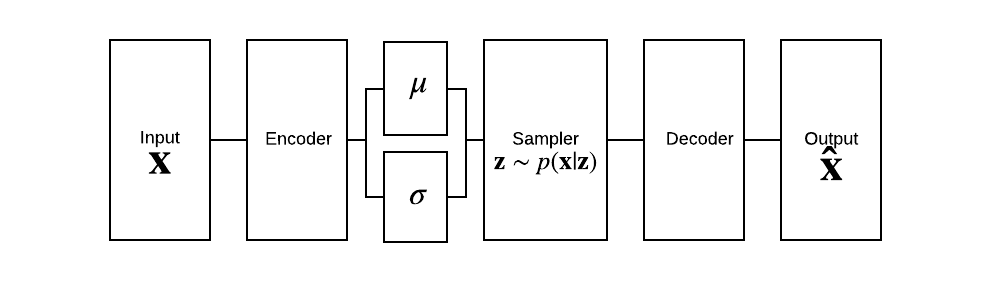
\includegraphics[width=1\textwidth]{../../media/encoder.png}%
\caption{Basic architecture of a Variational Autoencoder}
\label{fig:Bench1}
\end{figure}

\begin{figure}[!htb]
    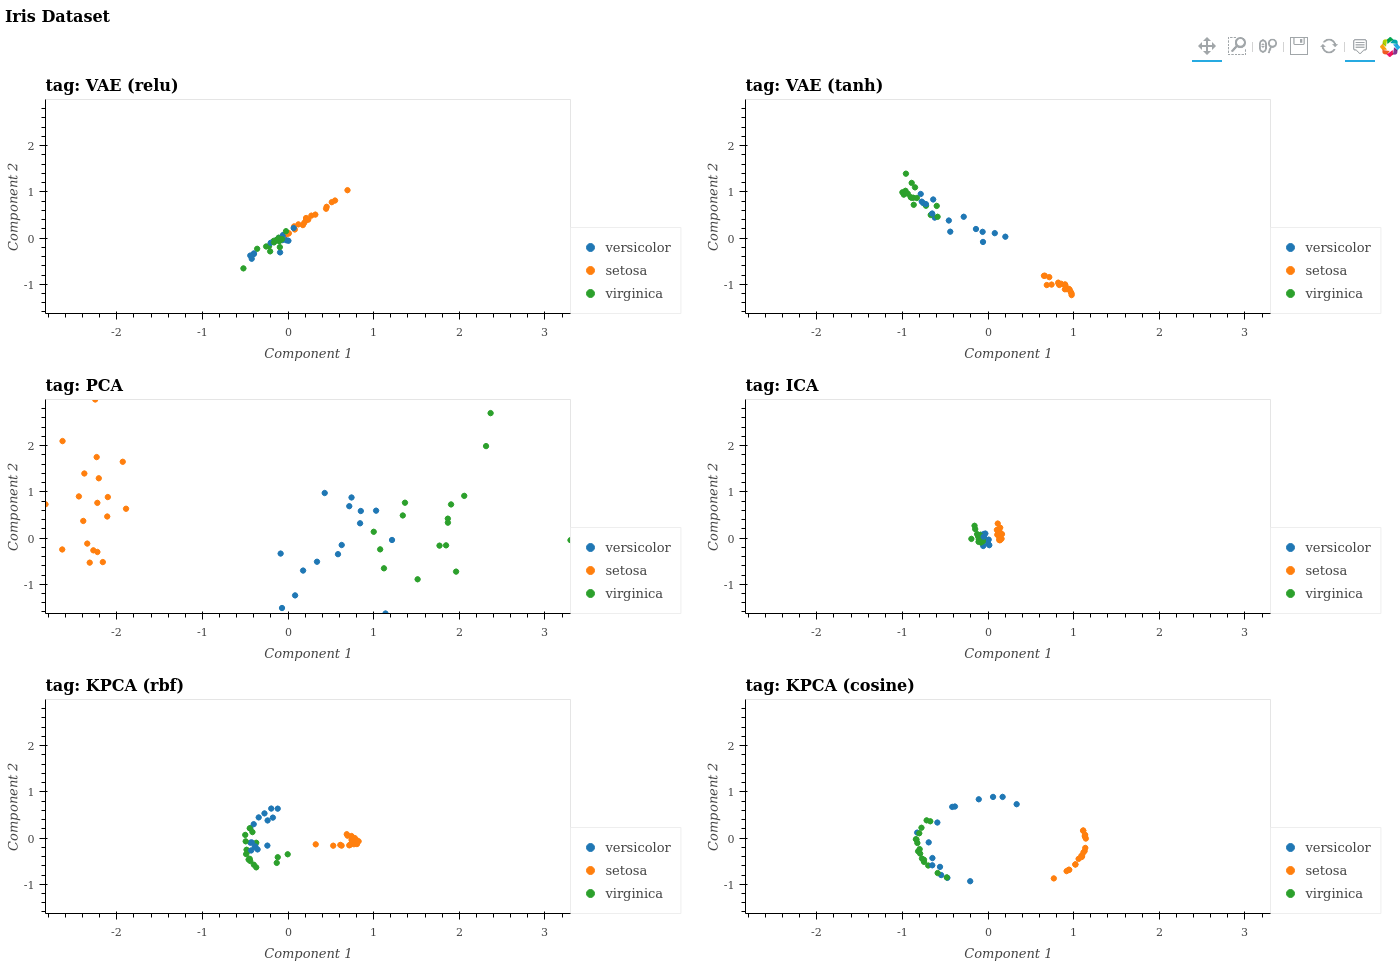
\includegraphics[scale=0.3]{../../media/02-iris-latent.png}
    \caption{Iris dataset Latent Space representation}
    \label{fig:benchirislatent}
\end{figure}

\begin{figure}[!htb]
    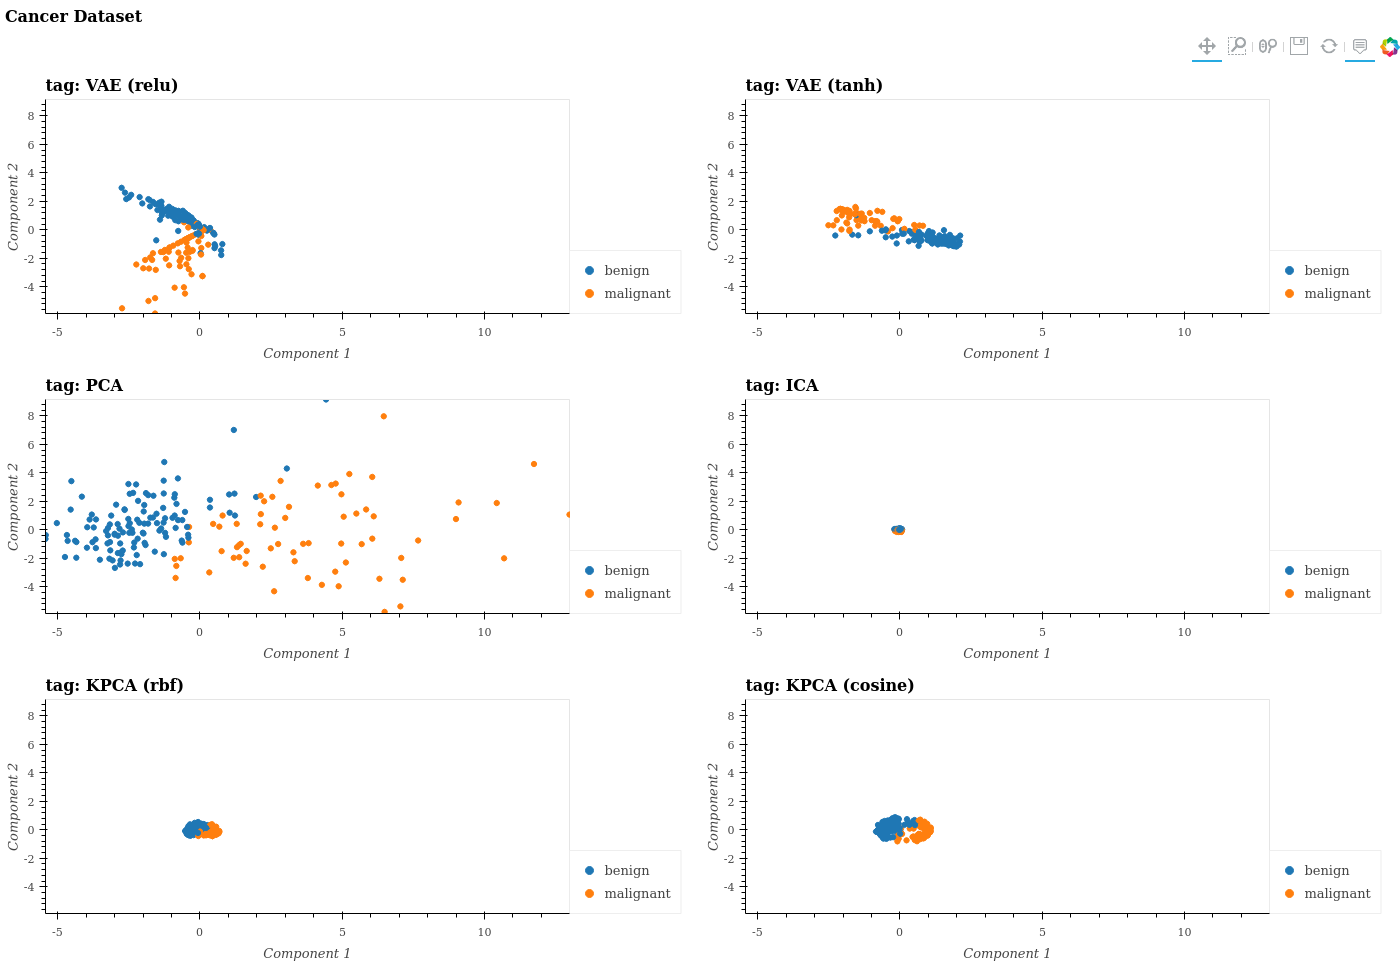
\includegraphics[scale =0.3]{../../media/02-cancer-latent.png}
    \caption{Cancer dataset Latent Space representation}
    \label{fig:benchcancerlatent}
\end{figure}


\begin{figure}[!htb]
    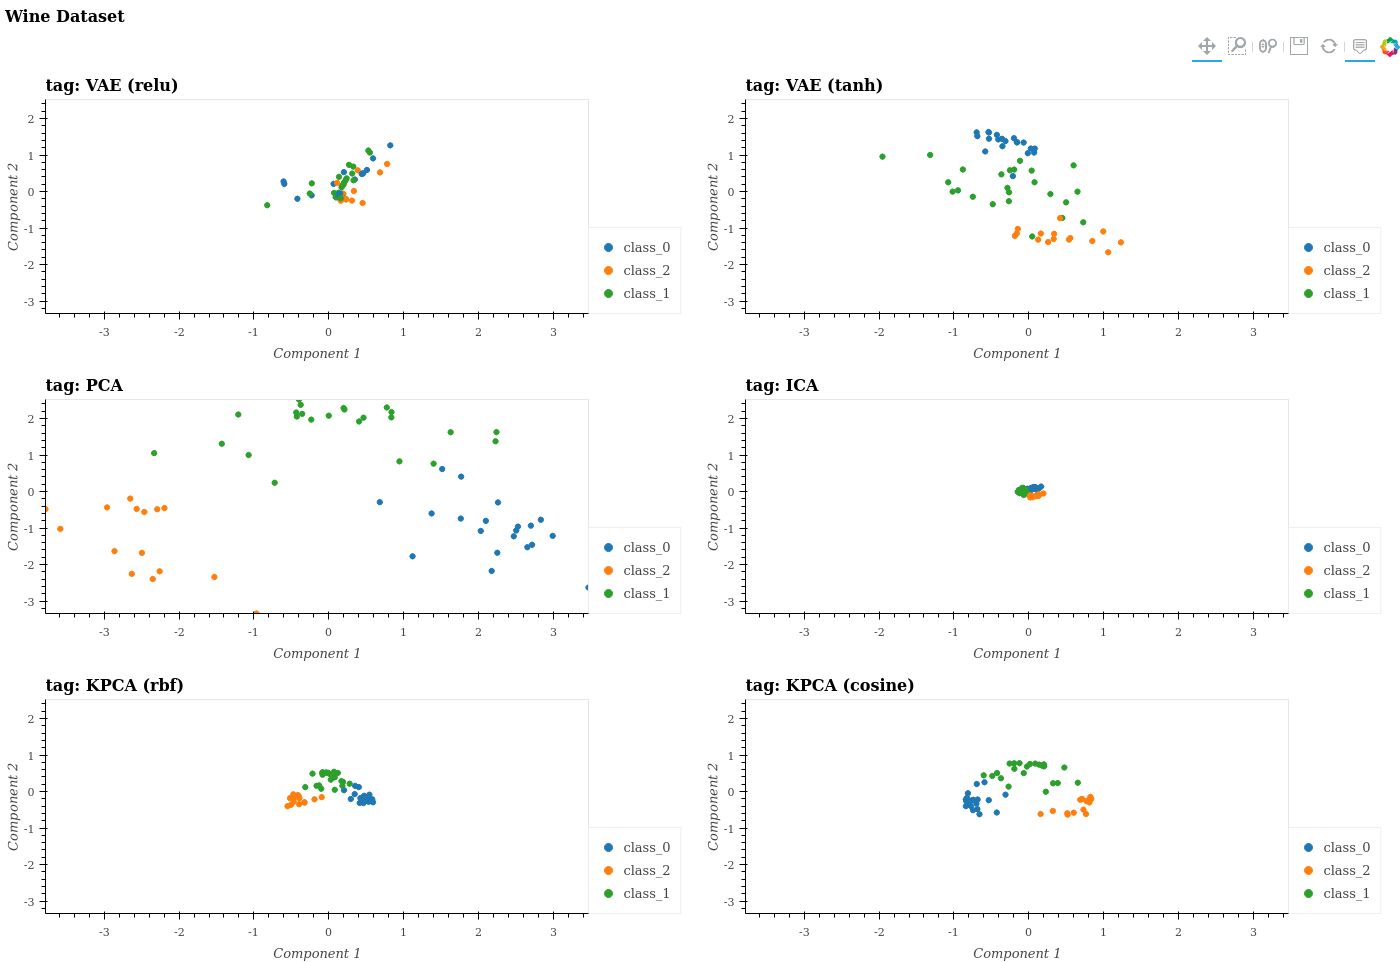
\includegraphics[scale=0.3]{../../media/02-wine-latent.png}
    \caption{Wine dataset Latent Space representation}
    \label{fig:benchwinelatent}
\end{figure}

\begin{figure}[!htb]
         \centering
         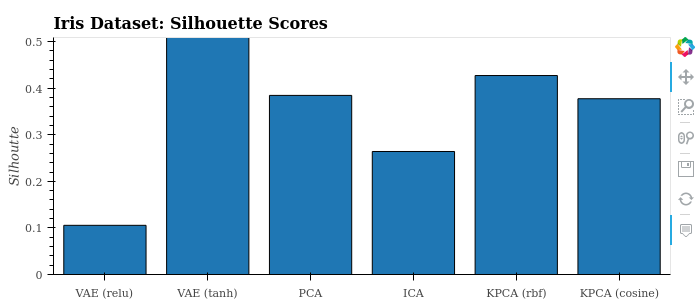
\includegraphics[scale=0.5]{../../media/02-iris-silhouette.png}
       
         \label{fig:benchiriss}
     
         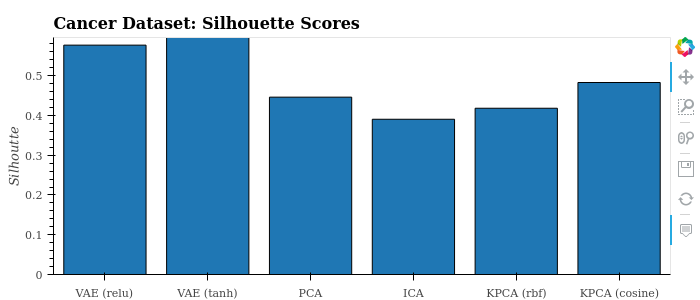
\includegraphics[scale=0.5]{../../media/02-cancer-silhouette.png}
     
         \label{fig:benchcancers}
     
         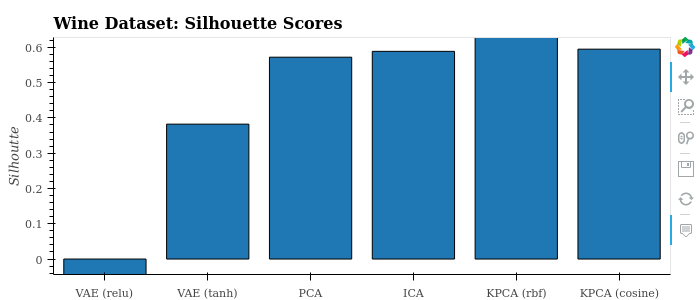
\includegraphics[scale=0.5]{../../media/02-wine-silhouette.png}

         \label{fig:benchwines}
        \caption{Silhouette Scores}
        \label{fig:clustering}
\end{figure}


\newpage


\subsection{Manifold Learning}
\begin{figure}[!htb]
    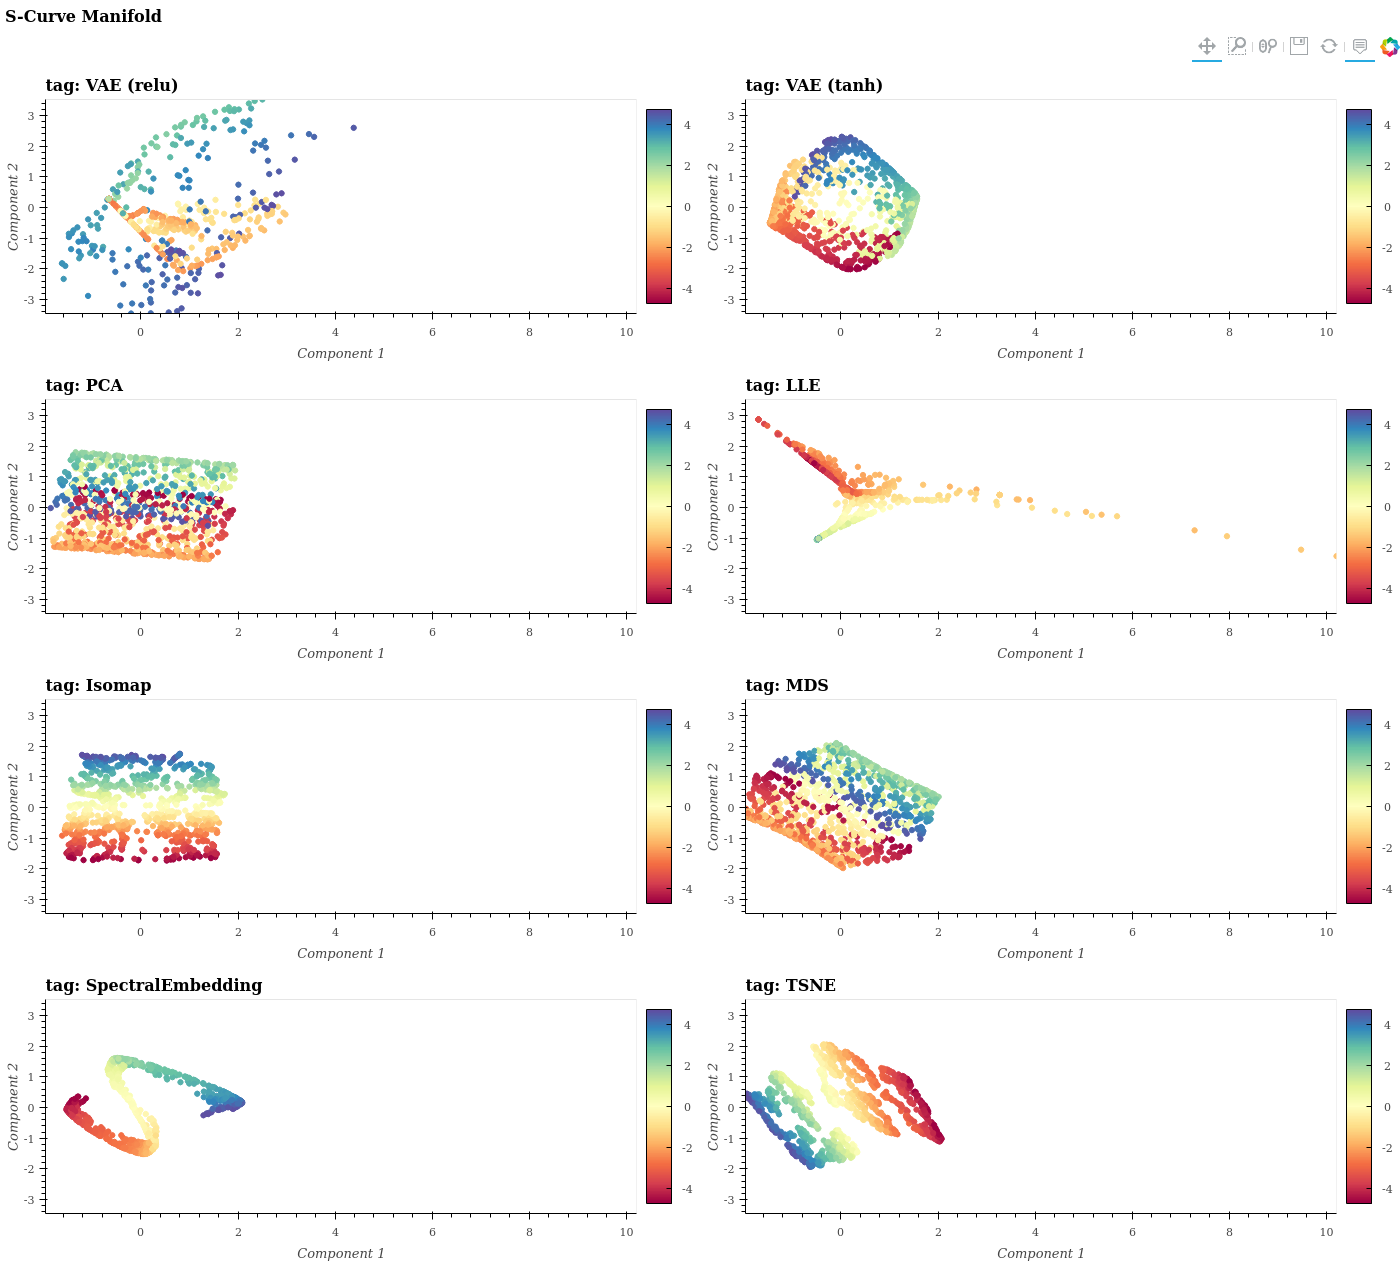
\includegraphics[scale =0.3]{../../media/03-scurve-latent.png}
    \caption{S-Curve Manifold Learning}
    \label{fig:scurve}
\end{figure}


\begin{figure}[!hb]
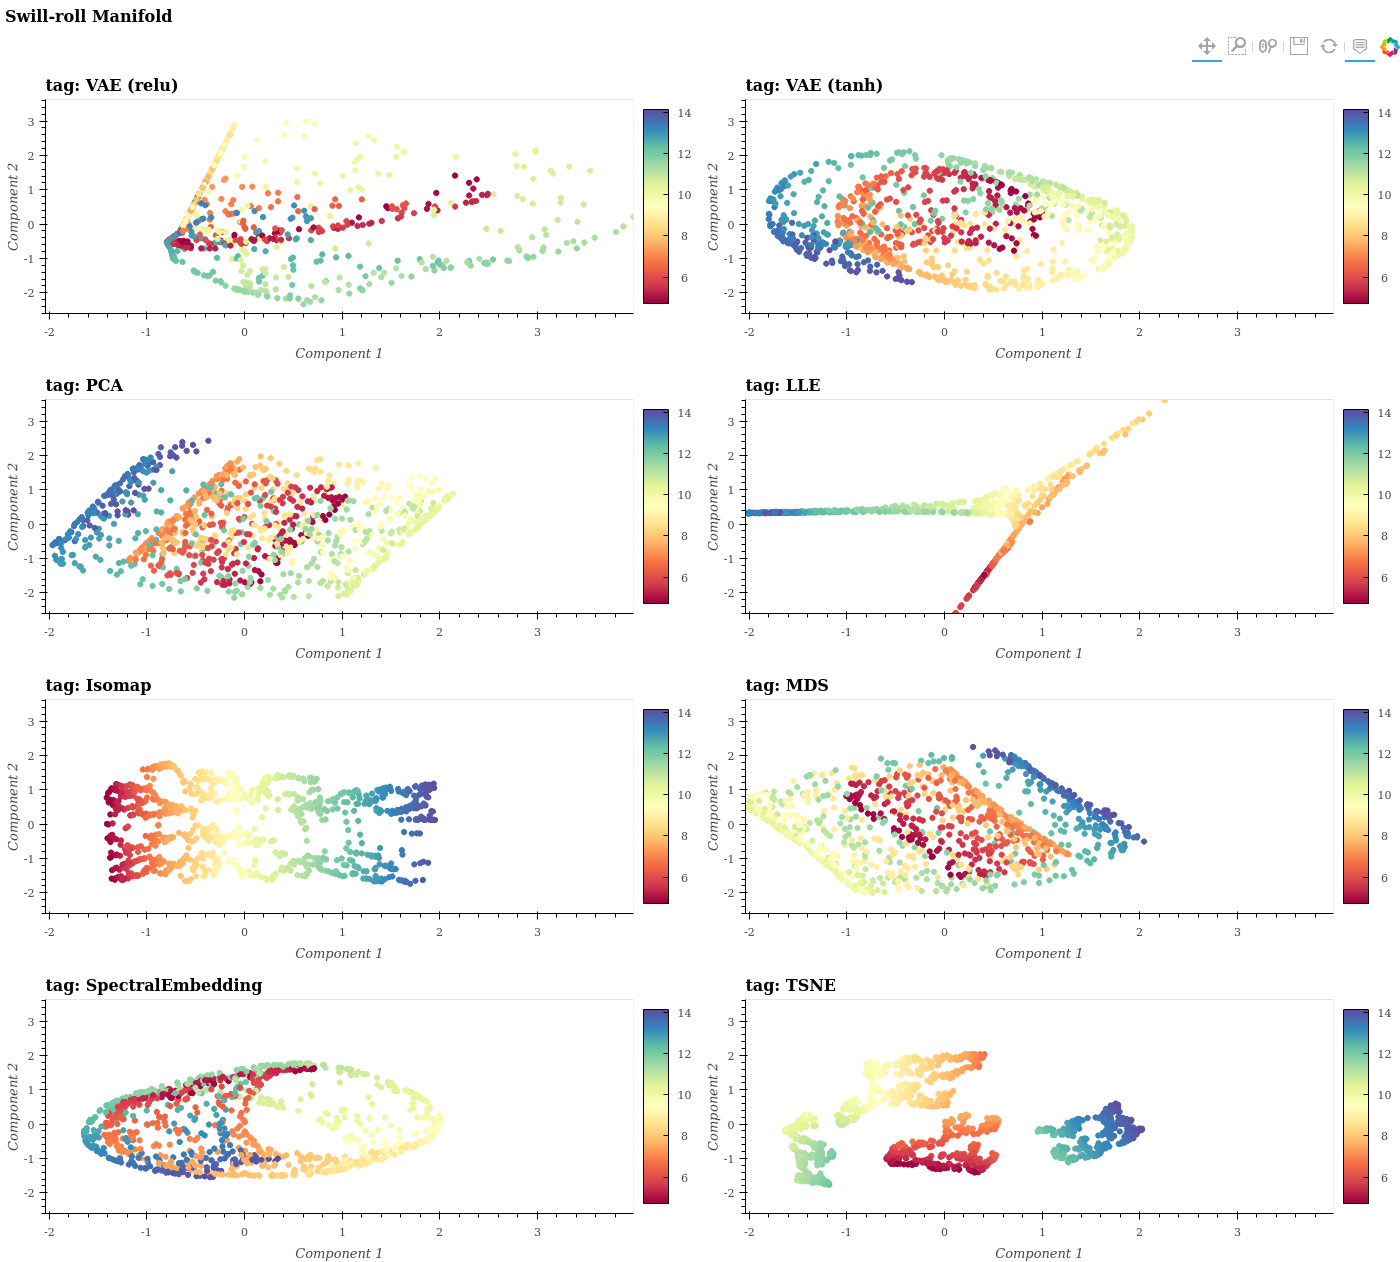
\includegraphics[scale = 0.3]{../../media/03-swissroll-latent.png}
    \caption{Swiss Roll manifold learning}
    \label{fig:swissroll}
\end{figure}

\newpage
\subsection{Heartbeats Audio}

\begin{figure}[!htb]
         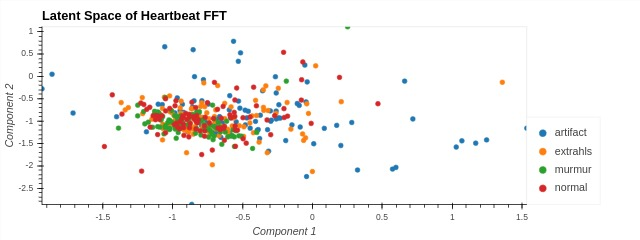
\includegraphics[scale=0.5]{../../media/heartbeat.jpeg}
       
         \label{fig:heart1}
     
         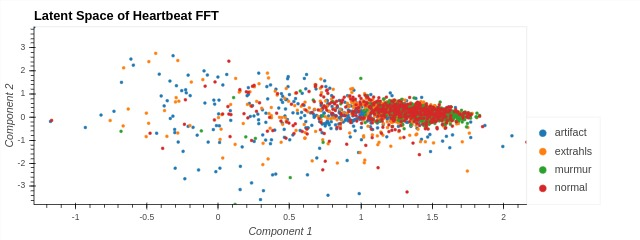
\includegraphics[scale=0.5]{../../media/heartbeat1.jpeg}
     
         \label{fig:heart2}
     
     
         \centering
         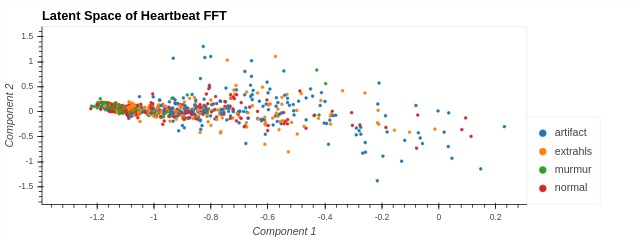
\includegraphics[scale=0.5]{../../media/heartbeat2.jpeg}

         \label{fig:heart3}
        \caption{Heartbeat Latent Space Representation}
        \label{fig:hearts}
\end{figure}

\newpage
\subsection{Generative Sampling}
\hspace{0.5em}
\begin{figure}[!htb]
     \centering
         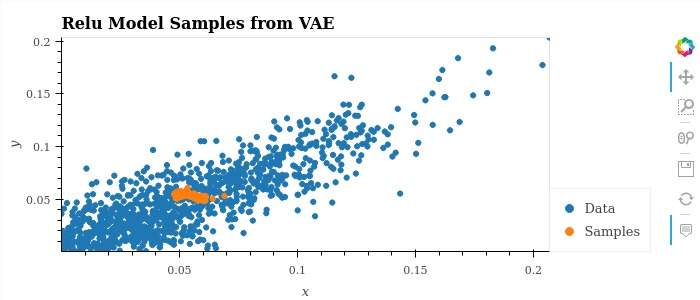
\includegraphics[scale=0.4]{../../media/generate.jpeg}
       
         \label{fig:gen1}
     
     
         \centering
         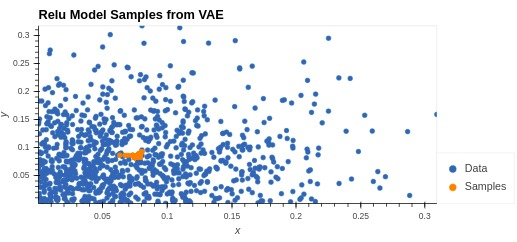
\includegraphics[scale=0.5]{../../media/generate3.jpeg}

         \label{fig:gen3}
        \caption{Gaussian Generative Modeling example}
        \label{fig:generative}
\end{figure}

\newpage

\begin{figure}[!hb]
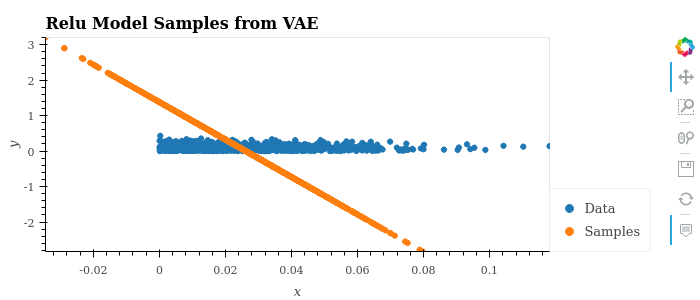
\includegraphics[scale = 0.3]{../../media/04-generative-pca.png}
    \caption{PCA on Bivariate Gaussian Generative Modeling example}
    \label{fig:generative-pca}
\end{figure}

\begin{figure}[!hb]
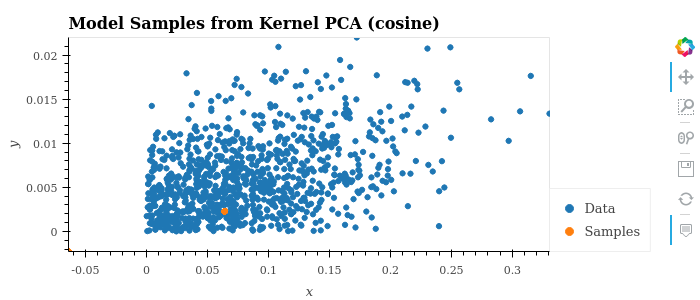
\includegraphics[scale = 0.3]{../../media/04-generative-kpca.png}
    \caption{Cosine Kernel PCA on Bivariate Gaussian Generative Modeling}
    \label{fig:generative-kpca}
\end{figure}
\newpage



\newpage
%\subsection{Code}
%\nocite{Basquin2018, Scipy, scikit-learn}
%\subsubsection{Exploratory Analysis}
%\lstinputlisting[language=Python]{../../notebooks/01-marcusinthesky-Exploration.py}
%\subsubsection{Dataset Benchmark Code}
%\lstinputlisting[language=Python]{../../notebooks/02-marcusinthesky-Reconstruction.py}
\subsubsection{Manifold Learning Comparison}
\lstinputlisting[language=Python]{../../notebooks/03-marcusinthesky-Manifold.py}
\subsubsection{Latent Space Sampling}
\lstinputlisting[language=Python]{../../notebooks/04-marcusinthesky-Sampling.py}
\subsubsection{Heartbeats Dataset}
\lstinputlisting[language=Python]{../../notebooks/05-marcusinthesky-Heartbeats.py}
\subsubsection{Library Code}
\lstinputlisting[language=Python]{../../super_spirals/io.py}
\lstinputlisting[language=Python]{../../super_spirals/metrics.py}
\lstinputlisting[language=Python]{../../super_spirals/neural_network.py}



\newpage
%\subsection{Environment}
%\lstinputlisting{../../environment.yml}

\bibliographystyle{bibstyle}
\bibliography{biblist}

\end{document}